\documentclass[tikz]{standalone}
\usetikzlibrary{positioning}

\begin{document}
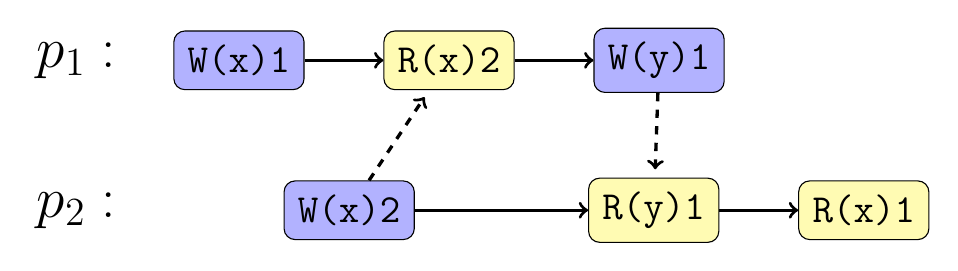
\begin{tikzpicture}
\tikzset{
  wop/.style = {rectangle, rounded corners, fill = blue!30, draw, font = \Large, inner sep = 5pt},
  rop/.style = {rectangle, rounded corners, fill = yellow!30, draw, font = \Large, inner sep = 5pt}, process/.style = {font = \huge}, po/.style = {->, very thick},
  rw/.style = {->, shorten >= 3pt, very thick, dashed},
  vis/.style = {->, shorten >= 3pt, very thick, dashed}
}

  \node (p1) [process] {$p_1:$};
  \node (wx1) [wop, right = 0.6cm of p1] {\texttt{W(x)1}};
  \node (rx2) [rop, right = 1cm of wx1] {\texttt{R(x)2}};
  \node (wy1) [wop, right = 1cm of rx2] {\texttt{W(y)1}};

  \node (p2) [process, below = 1.2cm of p1] {$p_2:$};
  \node (wx2) [wop, right = 2cm of p2] {\texttt{W(x)2}};
  \node (ry1) [rop, right = 2.2cm of wx2] {\texttt{R(y)1}};
  \node (rx1) [rop, right = 1cm of ry1] {\texttt{R(x)1}};

  \draw [po] (wx1) to (rx2);
  \draw [po] (rx2) to (wy1);

  \draw [po] (wx2) to (ry1);
  \draw [po] (ry1) to (rx1);

  \draw [vis] (wy1) to (ry1);
  \draw [vis] (wx2) to (rx2);

\end{tikzpicture}
\end{document}